%%%%%%%%%%%%%%%%%%%%%%%%%%%%%%%%%%%%%%%%%
%
% (c) 2024 by Jennifer Laaser
%
% This work is licensed under the Creative Commons Attribution-NonCommercial-ShareAlike 4.0 International License. To view a copy of this license, visit http://creativecommons.org/licenses/by-nc-sa/4.0/ or send a letter to Creative Commons, PO Box 1866, Mountain View, CA 94042, USA.
%
% The current source for these materials is accessible on Github: https://github.com/jlaaser/pogil-polymers
%
%%%%%%%%%%%%%%%%%%%%%%%%%%%%%%%%%%%%%%%%%

\renewcommand{\figpath}{content/polymphys/scattering/light-scattering/figs}
\renewcommand{\labelbase}{light-scattering}

\begin{activity}{Static and Dynamic Light Scattering}
\label{\labelbase}

\begin{instructornotes}
	This activity introduces students to concepts related to static and dynamic light scattering from polymer solutions.
	
	After completing this activity, students will be able to:
	\begin{enumerate}
		\item \dots
	\end{enumerate}
	
	\subsection*{Activity summary:}
	\begin{itemize}
		\item \textbf{Activity type:} Learning Cycle
		\item \textbf{Content goals:} See above 
		\item \textbf{Process goals:} %https://pogil.org/uploads/attachments/cj54b5yts006cklx4hh758htf-process-skills-official-pogil-list-2015-original.pdf
			\begin{enumerate}
				\item Interpretation of graphical data
				\item Written and oral communication of reasoning
			\end{enumerate}
		\item \textbf{Duration:} TBD minutes, including time for class discussion
		\item \textbf{Instructor preparation required:} none beyond knowledge of relevant content
		\item \textbf{Related textbook chapters:}
			\begin{itemize}
				\item \emph{Polymer Chemistry} (Hiemenz \& Lodge): section XX
				\item \emph{Introduction to Polymers} (Young \& Lovell): section YY
			\end{itemize}
		%\item \textbf{Instructor notes:}
		%	\begin{itemize}
		%		\item \dots
		%	\end{itemize}
	\end{itemize}
	
\end{instructornotes}

%%%%% REMOVING MODEL 1 FOR NOW - DON'T HAVE TIME TO FINISH IT FOR CLASS ON 4/2, but should complete this before adding to the formal collection, or move it to an extension, if the activity stands alone without it?

%\begin{model}[Interaction of Light with Molecules]
%	\label{\labelbase:mdl:lightmolecule}
%	
%	When a molecule is placed into an electric field, its electron cloud distorts (polarizes) to form an induced dipole, as shown below:
%	
%	IMAGE
%	
%	The greater the polarizability of the molecule, $\alpha$, the easier it is for the electric field to move the electrons around, and the larger the induced dipole.
%
%\end{model}
%
%\begin{ctqs}
%
%	\question Sketch the configuration of the electron cloud when the molecule is placed in each of the following fields:
%	
%		IMAGES
%		
%	\question The oscillating field in the previous problem creates an oscillating dipole.  Plot the dipole moment as a function of time on the following axes:
%	
%		AXES
%		
%%	\question Some molecules are easy to polarize (e.g. they don't hold onto their electrons very tightly, so it is easy for the electric field to move them around), while others are hard to polarize.  
%%	
%%		How would the dipole moment you plotted in the previous question differ if the molecule was very hard to polarize?  Sketch your answer on the following axes:
%%		
%%		AXES
%		
%	\question An oscillating dipole creates its \emph{own} oscillating electric field, which can be the source of a new electromagnetic wave (i.e. scattered light!).  %Why does this mean that polarizable molecules can scatter light?  
%	Do you expect the intensity of the scattered light to increase or decrease as you increase the polarizability of the molecule?   Explain your group's reasoning in 2-3 complete sentences.  \label{\labelbase:ctq:polarizability}
%
%%%%%% Move this to exercises, and/or solution of previous Q (for instructor to discuss)
%%\begin{infobox}
%%
%%	If light with wavelength $\lambda$ and intensity $I_0$ is incident on a molecule with polarizability $\alpha$, the intensity of the scattered light $I_s$ is
%%	\begin{equation*}
%%		\frac{I_s}{I_0} = \frac{16 \alpha^2 \pi^4}{r^2 \lambda^4}
%%	\end{equation*}
%%	where $r$ is the distance from the molecule to the detector.
%%\end{infobox}
%		
%	\question In light scattering experiments, the polymers of interest are usually dissolved in a solvent.
%	
%		\begin{enumerate}	
%			\item \dots 
%		\end{enumerate}
%		
%	\question Explain, in 2-3 complete sentences, why we usually analyze the \emph{excess scattering}, $\dots$.  % could move to end and get them to the idea of dn/dc?
%	
%	\question In light scattering experiments, the wavelength of light is usually much longer than the size of the particles or the distances between them.
%	
%		GET AT IDEA THAT IT IS THE AVERAGE POLARIZABILITY THAT MATTERS - and then connect to refractive index?
%	
%\end{ctqs}



\begin{model}[Incoherent Scattering]
	
	If the distribution of molecules in a sample is perfectly homogeneous, then every molecule has a ``partner'' that is exactly the right distance away to scatter light with a phase difference of $\delta = \pi$, as shown below:
	
	\centerline{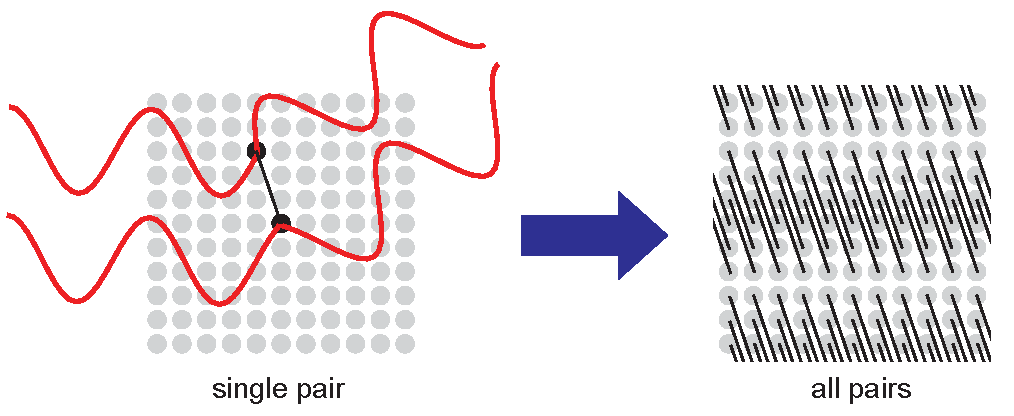
\includegraphics[width=0.75\textwidth]{\figpath/Model1_pairing}}
	
\end{model}


\begin{ctqs}
	
	\question Will any scattered intensity be observed in a light scattering measurement on a perfectly homogeneous sample?  Why or why not?  Explain your group's reasoning in 1-2 complete sentences.
	
		\begin{solution}[1.5in]
		\end{solution}

	\question Suppose one of the molecules is moved, as shown below.
	
	\vspace{6pt}
	\centerline{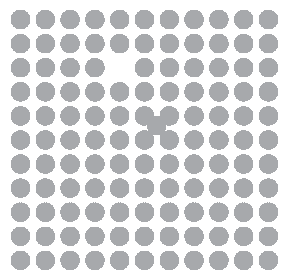
\includegraphics[width=0.2\textwidth]{\figpath/Model1_displacement}}

		\begin{enumerate}
			\item Do the molecules all still have ``partners'' that are the right distance away to scatter light with perfect destructive interference? 
	
		\begin{solution}[0.5in]
		\end{solution}
			
			\item Will any scattered intensity be observed in a light scattering measurement on this sample?  Why or why not?  Explain your group's reasoning in 1-2 complete sentences.
	
		\begin{solution}[1in]
		\end{solution}
			
		\end{enumerate}
		
	\question Several possible distributions of molecules in a sample are shown below: \label{\labelbase:ctq:fluctuations}
	
	\centerline{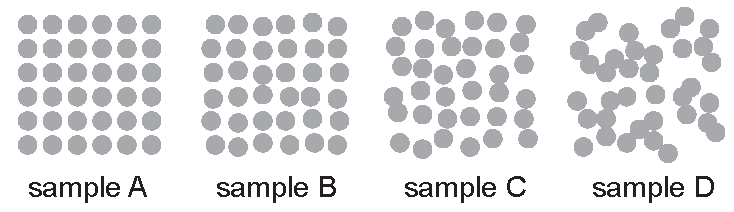
\includegraphics[width=0.5\textwidth]{\figpath/Model1_fluctuation}}
	
		Which of these samples would you expect to give the \emph{highest} intensity of scattered light?  Explain your group's reasoning in 1-2 complete sentences.
	
		\begin{solution}[1in]
		\end{solution}

\end{ctqs}

\begin{infobox}
	It is possible to show that the excess scattering from a polymer sample is related to the size of the concentration fluctuations in cells of volume $\Psi$ by
	\begin{equation*}
		\frac{I_{ex}}{I_0} = \frac{4 \pi^2 n^2 \Psi}{r^2 \lambda^4}\left(\frac{\partial n}{\partial c}\right)^2_{T,p} \langle ( \delta c )^2 \rangle
	\end{equation*}
	Here, $\delta c$ is the size of the concentration fluctuations, and $\frac{d n}{dc}$ is the change in the refractive index of the mixture with changes in the solute concentration $c$ (where $c$ is measured in units of mass of solute per unit volume).
\end{infobox}

\begin{ctqs}

	\question Is this expression consistent with your answer to CTQ \ref{\labelbase:ctq:fluctuations}?  Briefly explain how you know.
	
		\begin{solution}[1in]
		\end{solution}
	
\end{ctqs}

\begin{model}[Equilibrium Fluctuations \& Static Light Scattering]
	\label{\labelbase:mdl:SLS}

Changes in polymer concentration typically change the free energy of the mixture, as shown below.
	
	\centerline{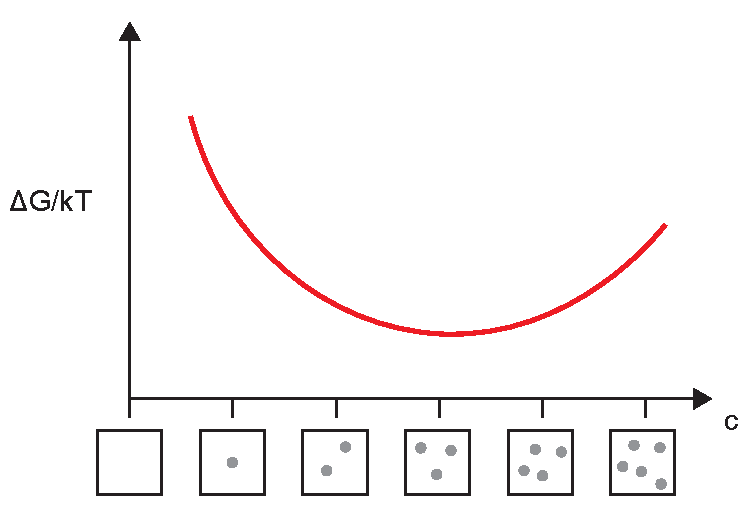
\includegraphics[width=0.4\textwidth]{\figpath/Model1_deltaG}}
	
\end{model}

\begin{ctqs}
	
		\question Which of the following two states has the higher free energy?
	
	\vspace{6pt}
	\centerline{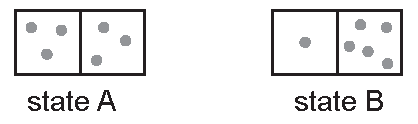
\includegraphics[width=0.3\textwidth]{\figpath/Model1_twostates}}
	
			\begin{solution}[0.25in]
			\end{solution}
			
		\question For which of the following free energy curves will it be ``easiest'' to go from state A to state B?  Briefly explain your reasoning.  \label{\labelbase:ctq:delGcurvature}
	
	\centerline{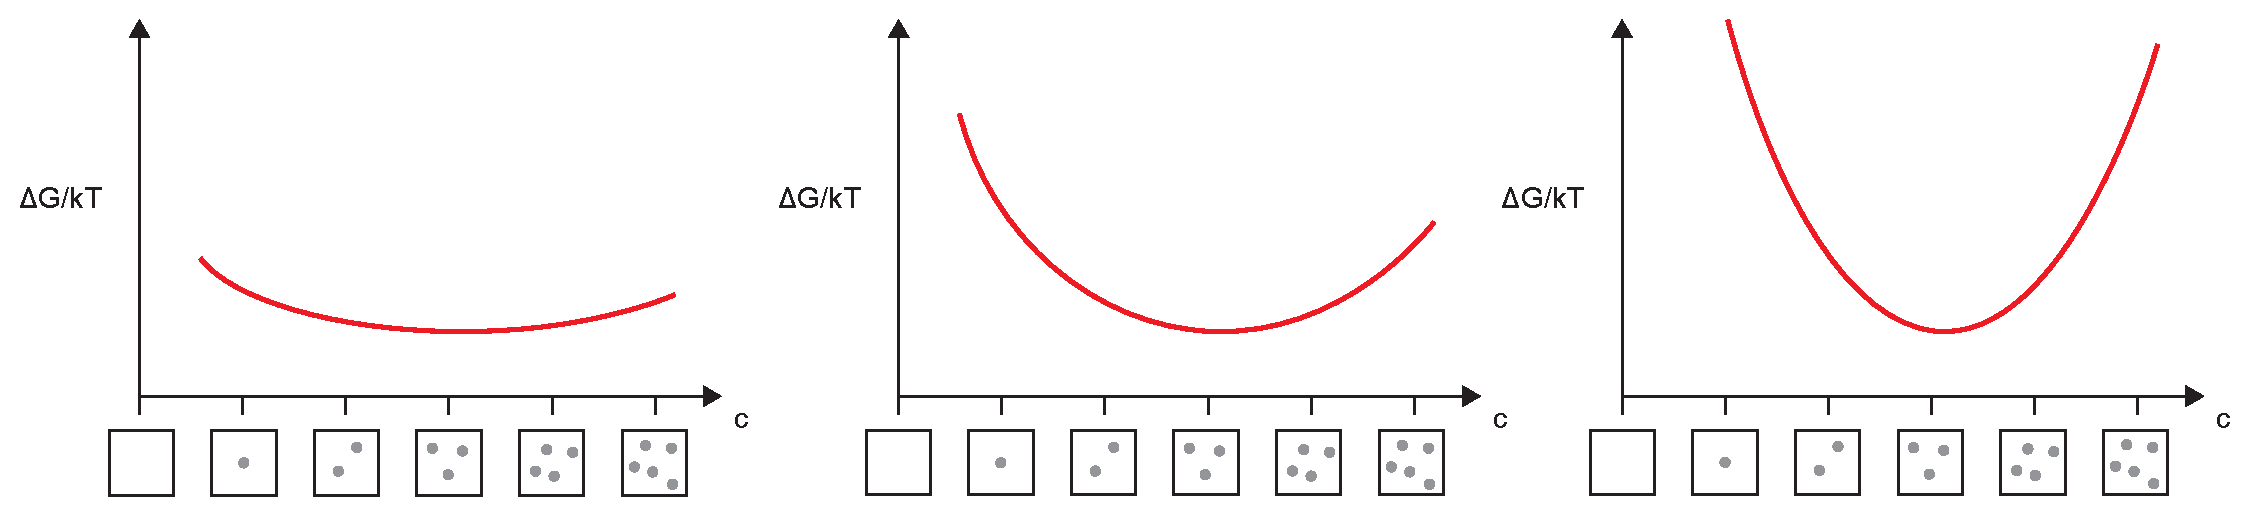
\includegraphics[width=0.8\textwidth]{\figpath/Model1_curvature}}
	
			\begin{solution}[1in]
			\end{solution}
			
	\question If the temperature of the system is increased, will it be easier or harder to go from state A to state B?  Briefly explain your reasoning. \label{\labelbase:ctq:temperature}
	
			\begin{solution}[1in]
			\end{solution}
	
\end{ctqs}

\begin{infobox}
	It is possible to show that the average size of the concentration fluctuations across cells of volume $\Psi$ is
	\begin{equation*}
		\langle (\delta c)^2\rangle = \frac{k_BT}{\left( \frac{\partial^2 G}{\partial c^2}\right)_{T,p}} = \frac{c}{\Psi N_{av}} \frac{1}{1/M_w + 2Bc + \dots}
	\end{equation*}
	where $M_w$ is the weight-average molecular weight of the polymer and $B$ is the so-called ``second virial coefficient'' which reflects how much the polymer chains do or do not prefer to be near other polymers in solution.
\end{infobox}

\begin{ctqs}
	\question Is this expression consistent with the behavior you predicted in CTQs \ref{\labelbase:ctq:delGcurvature} and \ref{\labelbase:ctq:temperature}?  Briefly explain how you know.
	
		\begin{solution}[1in]
		\end{solution}

	\question Combine the equations from the two preceding Information boxes to obtain one (messy!) equation for $I_{ex}/I_0$.   Don't worry about simplifying it, but do verify that the $\Psi$ terms cancel out.
	
		\begin{solution}[1.5in]
			\begin{align*}
				\frac{I_{ex}}{I_0} &= \frac{4 \pi^2 n^2 \Psi}{r^2 \lambda^4}\left(\frac{\partial n}{\partial c}\right)^2_{T,p} \frac{c}{\Psi N_{av}} \frac{1}{1/M_w + 2Bc + \dots} \\
				&= \frac{4 \pi^2 n^2}{r^2 \lambda^4}\left(\frac{\partial n}{\partial c}\right)^2_{T,p} \frac{c}{ N_{av}} \frac{1}{1/M_w + 2Bc + \dots}
			\end{align*}
		\end{solution}
		
	\question It is usually convenient to group all of the constants into a single optical constant, $K$, where
		\begin{equation*}
			K = \frac{4\pi^2 n^2 (\partial n / \partial c)^2}{\lambda^4 N_{av}}
		\end{equation*}
		Rewrite your expression for $\frac{I_{ex}}{I_0}$ in terms of the optical constant $K$, the concentration of the polymers $c$, their molecular weight $M_w$, and the second virial coefficient, $B$.
		
		\begin{solution}[1in]
			\begin{equation*}
				\frac{I_{ex}}{I_0} = \frac{Kc}{r^2} \frac{1}{1/M_w + 2Bc + \dots}
			\end{equation*}
		\end{solution}
	
	\question It is also often most convenient to work in terms of the \emph{Rayleigh ratio}, $R_\theta = \frac{r^2 I_{ex}}{I_0}$.  Rearrange your answer from the previous question to obtain an expression for $R_\theta$.
		
		\begin{solution}[1in]
			\begin{equation*}
				R_\theta = r^2 \frac{I_{ex}}{I_0} = \frac{Kc}{1/M_w + 2Bc + \dots}
			\end{equation*}
		\end{solution}
	
	
\end{ctqs}

\begin{infobox}

	Polymers are not quite point particles, so the light scattered from each polymer chain in the sample has a small dependence on $q$.  If $qR_g < 1$, then the $q$-dependence is given by the form factor,
	\begin{equation*}
		P(q) = 1 - \frac{q^2}{3}R_g^2 + \dots
	\end{equation*}
	Combining this with the expression you obtained in the previous question, we find that
	\begin{equation*}
		\frac{Kc}{R_\theta} = \frac{1}{M_w}\left( 1 + \frac{q^2}{3} R_g^2 + \dots \right) + 2Bc + \dots
	\end{equation*}
	This is the \emph{Zimm equation}.
\end{infobox}

\begin{ctqs}
	
	\question When $c$ is very small,
		\begin{equation*}
			\frac{Kc}{R_\theta} \approx \frac{1}{M_w}\left(1 + \frac{q^2}{3}R_g^2 + \dots\right)
		\end{equation*}
		Propose a method that you could use to determine \emph{both} the weight-average molecular weight \emph{and} the radius of gyration of a polymer from data about how the intensity of light scattered from a dilute polymer solution changes with scattering angle.
		
		\begin{solution}[2.5in]
		\end{solution}
		
	\question If you wanted to additionally obtain information about the second virial coefficient, $B$, how would you modify your proposed experiment?  Explain your reasoning in 1-2 complete sentences.
		
		\begin{solution}[1.5in]
		\end{solution}
		
\end{ctqs}


\begin{model}[Time-Dependent Fluctuations and Dynamic Light Scattering]
	\label{\labelbase:mdl:DLS}
	
	In Model \ref{\labelbase:mdl:SLS}, above, we considered only the \emph{average} intensity of the light scattered from a polymer solution.   However, the distribution of molecules (and the scattered intensity) can also change with time.
	
	Shown below are the distributions of molecules that might be present in a polymer solution at a series of different times, $t$:
	
	\vspace{6pt}
	\centerline{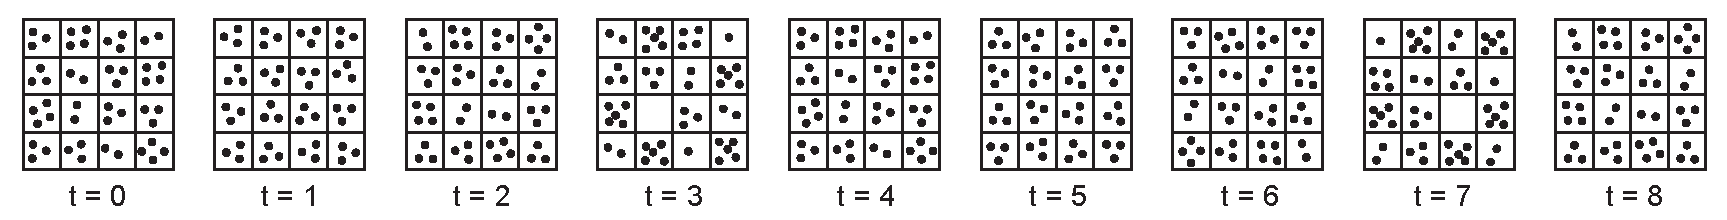
\includegraphics[width=\textwidth]{\figpath/Model2_fluctuations_medium}}
	
\end{model}

\begin{ctqs}

	\question At which times are the concentrations of molecules at different positions in the solution...
	
		\begin{enumerate}
			\item ... very similar?
			
				\begin{solution}[0.25in]
				\end{solution}
			
			\item ... very different?
			
				\begin{solution}[0.25in]
				\end{solution}
		\end{enumerate}
		
	\question At which times will the solution...
	
		\begin{enumerate}
			\item ... scatter a lot of light?
			
				\begin{solution}[0.25in]
				\end{solution}
			
			\item ... scatter little light?
			
				\begin{solution}[0.25in]
				\end{solution}
				
		\end{enumerate}
		
		\clearpage
	\question On the following axes, sketch the intensity of the scattered light that you would expect to measure from this solution as a function of time:
	
		\vspace{6pt}
		\centerline{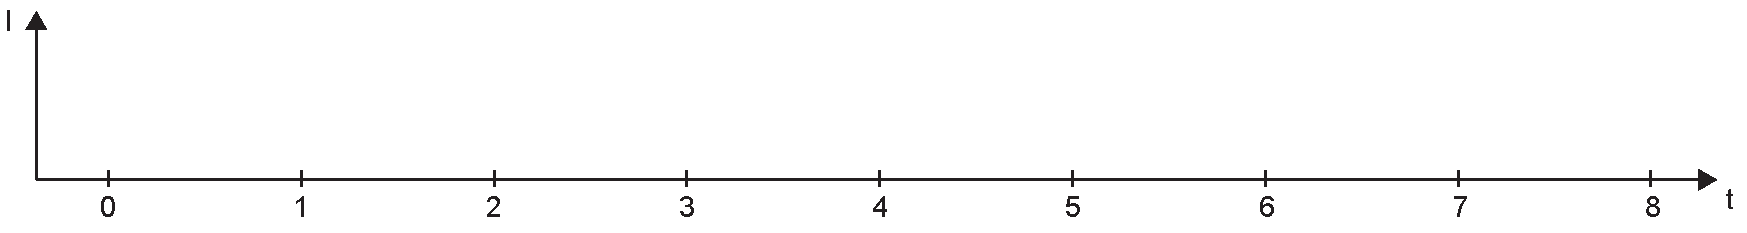
\includegraphics[width=0.9\textwidth]{\figpath/Model2_Is_blank}}
		\vspace{6pt}
		
	\question The time-dependent distributions of molecules in two different solutions are shown below.  For each solution, sketch the intensity of the scattered light that you would expect to measure from the solution as a function of time.
	
		\begin{enumerate}
			\item Solution A:
			
			\vspace{6pt}
			\centerline{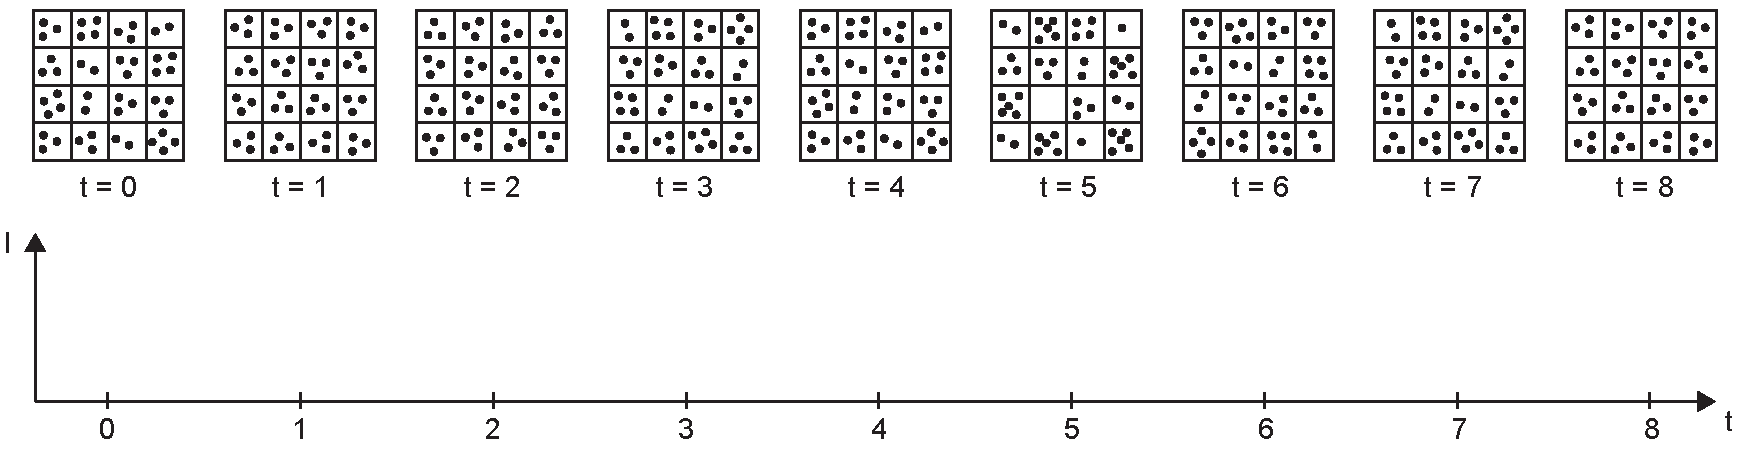
\includegraphics[width=0.9\textwidth]{\figpath/Model2_fluctuations_slow}}
			\vspace{6pt}
			
			\item Solution B:
			
			\vspace{6pt}
			\centerline{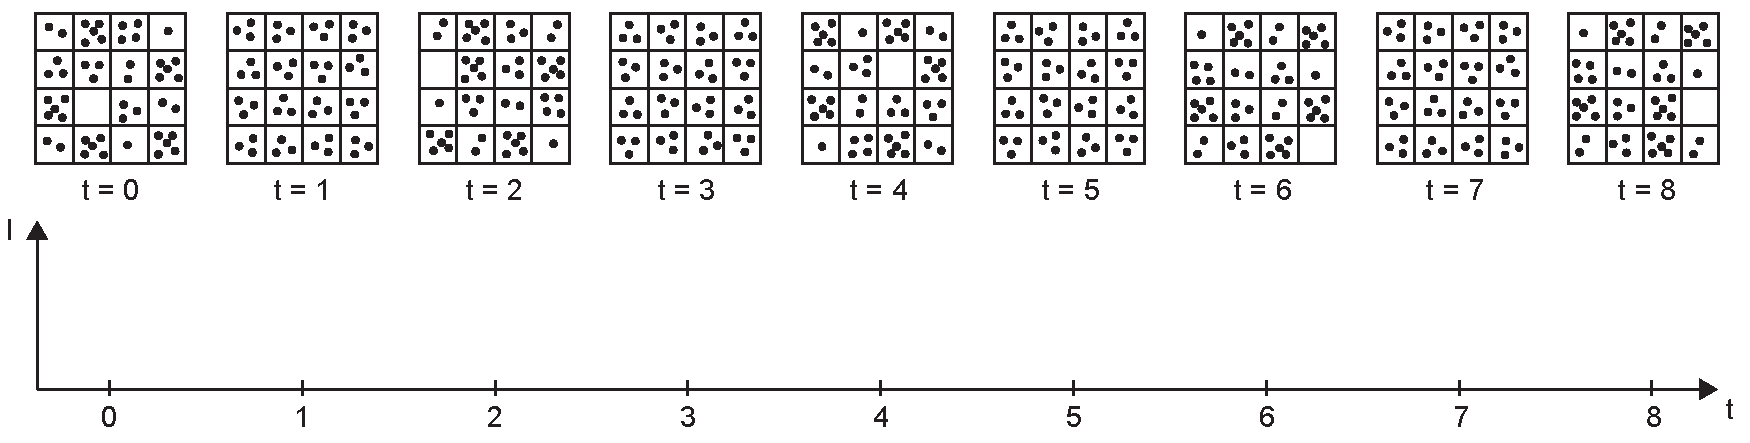
\includegraphics[width=0.9\textwidth]{\figpath/Model2_fluctuations_fast}}
		\end{enumerate}
		
	\question In which of the solutions shown above do you think the molecules were probably diffusing \emph{fastest}?  Explain your group's reasoning in 1-2 complete sentences.
	
		\begin{solution}[1.5in]
		\end{solution}
	
\end{ctqs}

\clearpage
\begin{infobox}
	The timescales over which the scattered intensities change can be characterized using the \textit{intensity autocorrelation function},
	\begin{equation*}
		C(t) = \int I_s(t') I_s(t'+t)dt'
	\end{equation*}
	For molecules diffusing with diffusion coefficient $D$, the intensity autocorrelation function measured at scattering vector $q$ has the form
	\begin{equation*}
		C(t) = A e^{-2 q^2 D t} + B
	\end{equation*}
\end{infobox}

\begin{ctqs}
	\question The intensity autocorrelation functions obtained from three different samples are shown below.
	
			\vspace{6pt}
			\centerline{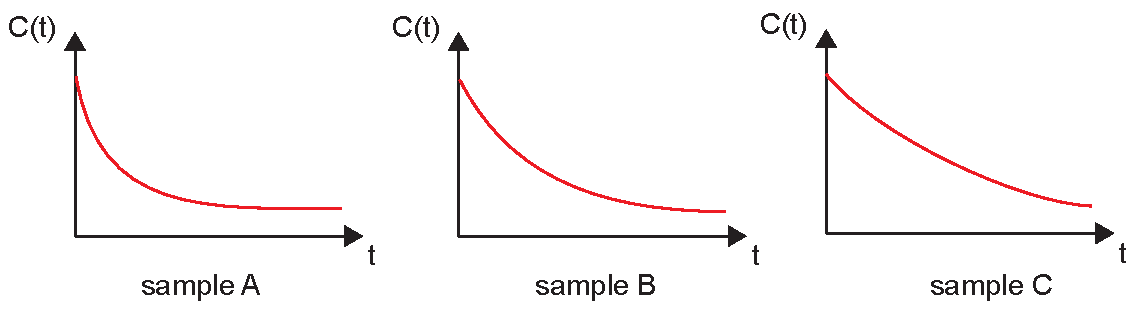
\includegraphics[width=0.7\textwidth]{\figpath/Model2_correlationfunctions}}	
	
		If all three samples were measured at the same scattering angle, in which sample were the particles diffusing the fastest?  Explain your reasoning in 1-2 complete sentences.
	
		\begin{solution}[1.25in]
		\end{solution}
	
	\question The diffusion coefficient of spherical particles with radius $R$ in a solvent with viscosity $\eta_s$ is given by the Stokes-Einstein relation,
	\begin{equation*}
		D = \frac{ k_B T}{6\pi \eta_s R}
	\end{equation*}
	Based on this relationship, in which of the samples in the preceding question must the particles have been the \emph{largest}?  Explain your reasoning in 1-2 complete sentences. \label{\labelbase:ctq:stokeseinstein}
	
		\begin{solution}[1.25in]
		\end{solution}
	
	\question Summarize, in your own words, how you could determine the effective radius of a polymer in solution from data about how the scattering intensity varies with time.
	
		\begin{solution}[1.5in]
		\end{solution}

\end{ctqs}



\begin{exercises}

	\exercise The Stokes-Einstein relation, as given in CTQ \ref{\labelbase:ctq:stokeseinstein}, assumes that the particle is a perfect sphere.
	
		\begin{enumerate}
		
			\item Are polymer chains perfectly spherical particles?  If not, how would you interpret the value of $R$ obtained in a dynamic light scattering experiment?  Explain why we typically refer to radii measured in this way as ``hydrodynamic'' radii.
			
			\item Is the hydrodynamic radius ($R_h$) of a polymer chain obtained in a dynamic light scattering experiment likely to be bigger or smaller than its radius of gyration ($R_g$)?  Explain your reasoning in 1-2 complete sentences.
			
		\end{enumerate}
	
\end{exercises}


%\begin{problems}
%
%	\problem First exercise
%	\problem Second exercise
%	
%\end{problems}


	
\end{activity}